\chapter{Background}
\label{chap:technical}

\section{The Lambda Calculus}
\newcommand{\lcalc}{$\lambda$-calculus}
\newcommand{\lCalc}{$\lambda$-Calculus}
\newcommand{\fto}{\rightarrow}
The lambda calculus (\lcalc) was described by Alonzo Church in 1936~\cite{church1936unsolvable}. It is a universal model of computation, meaning we can implement any Turing machine using it, meaning we can compute any computable function using it \cite{Turing_1937}. The \lcalc\ is important because it provides a foundation for functional programming languages. Understanding the \lcalc\ is essential for understanding the principles behind these languages and how they evaluate expressions.

The set of all lambda terms is $\Lambda$. Lambda calculus is built from three syntax structures:
\begin{itemize}
    \item Variables, selected from an infinite set of variables $V=\{x,y,z,\dots\}$
    \item Abstractions, $\lambda x. M$ which are functions, where we `bind' a variable $x$ for use in the term $M$ such that when we apply our function to a term $N$, all instances of $x$ in $M$ are substituted with $N$.
    \item Applications $M N$ where we apply a term $M$ to an argument $N$. 
\end{itemize}

\noindent Below is a more formal definition of the \lcalc~\cite{barendregt2013lambda}.
\begin{alignat*}{3}
&x \in V                 \quad && \implies \quad && x \in \Lambda               \\
&M,N \in \Lambda         \quad && \implies \quad && (M N) \in \Lambda           \\
&M \in \Lambda, x\in V   \quad && \implies \quad && (\lambda x. M) \in \Lambda  
\end{alignat*}

\noindent We shall also use the following fairly standard conventions:

\begin{enumerate}
    \item Application is left associative. The term $M_1\,M_2\,M_3$ means $(M_1\,M_2)\,M_3$ and not $M_1\,(M_2\,M_3)$
    \item Nested abstractions can be grouped: the term $\lambda x \;y. M$ means $(\lambda x . (\lambda\;y. M))$.
    \item Outermost parenthesis are omitted.
    \item The body of an abstraction extends as far to the right as possible: the term $\lambda x. M\,N$ means $(\lambda x. (M\;N))$ and not $((\lambda x. M)\,N)$. 
\end{enumerate}

\subsection{Free variables}
\begin{quotation}
\noindent`An occurrence of $x$ is free if it appears in a position where it is not bound by an enclosing abstraction on $x$' \cite{pierce2002types}
\end{quotation}

\noindent Free variables are a useful concept to express which variables are `ready for substitution' in a term. Formally, the function $FV(M)$ is the set of free variables in the term $M$ \cite{barendregt2013lambda}:
\begin{alignat*}{3}
FV(x)              \quad && = \quad && &\{x\}               \\
FV(M\,N)           \quad && = \quad && &FV(M)\union FV(N)   \\
FV(\lambda x. M)   \quad && = \quad && &FV(M)-\{x\}         \\
\end{alignat*}

\noindent A term is \textit{closed} if it has no free variables, and \textit{open} if it does. 

\subsection{Reduction}
\begin{quotation}
\noindent`The sole means by which terms `compute' is the application of functions to arguments (which themselves are functions). Each step in the computation consists of rewriting an application whose left-hand component is an abstraction, by substituting the right-hand component for the bound variable in the abstraction's body' \cite{pierce2002types} 
\end{quotation}

\noindent The \lcalc\ is evaluated by $\beta$-reduction. This is where an abstraction is applied to a value. The result of applying an abstraction to a term is the body of the abstraction, with the all free instances of the abstracted variable are substituted with the term the abstraction was applied to. Below is the definition of substitution within a term formally \cite{barendregt2013lambda}. 
\noindent\begin{alignat*}{3}
&x[x:=N]                        \quad && \equiv \quad && N                       \\
&y[x:=N] \text{ where } y \ne x \quad && \equiv \quad && y                       \\
&(M_1 M_2)[x:=N]                \quad && \equiv \quad && (M_1[x:=N]) (M_2[x:=N]) \\
&(\lambda y.M)[x:=N]            \quad && \equiv \quad && \lambda y.(M[x:=N])     
\end{alignat*}  
\noindent The definition of $\beta$-reduction \cite{barendregt2013lambda}:
\begin{alignat*}{3}
&x                 \quad && \BetaReduce \quad &&        x           \\
&\lambda x.M       \quad && \BetaReduce \quad &&        \lambda x.M \\
&(\lambda x.M) N   \quad && \BetaReduce \quad &&        M[x:=N]
\end{alignat*}
A term is said to be in \textbf{normal form} if it cannot be $\beta$-reduced. A term that can be beta reduced can be said to be a \textbf{redex} - reducible expression. The resulting term from reducing a redex is often called a \textbf{contraction}.

\subsection{Evaluation Strategies and Values}
We often have a term where we have multiple options for $\beta$-reduction. In this section, we will briefly discuss three different evaluation strategies that inform which option is selected when evaluation: call-by-value (a.k.a. strict), call-by-name and call-by-need (a.k.a. lazy). When a term is fully reduced under a given evaluation strategy, we say it is a value. I have used the same examples as Pierce \cite{pierce2002types}. For instance, the closed term 
\[(\lam{x} x)\,((\lam{x} x)\,(\lam{z} (\lam{x}. x) z))\] has three redexes ($id$ is shorthand for $\lam{x} x$):
\[\underline{id\,(id\,(\lam{z} id\,z))}\]
\[id\,\underline{(id\,(\lam{z} id\,z))}\]
\[id\,(id\,(\lam{z} \underline{id\,z}))\]

\noindent Most languages use the \textbf{call-by-value} evaluation strategy, where `only the outermost redexes are reduced and a redex is reduced only when its right-hand side has already been reduced to a value \ldots\ where the only values are \lambda expressions'\cite{pierce2002types}. This reduction strategy is also known as `strict'. Our chosen redex here would be number 2. We would reduce by the following sequence:
\begin{alignat*}{2}
id\,\underline{(id\,(\lam{z} id z))}  && \;\;\arr\\ 
(\underline{id\,(\lam{z} id z)})      && \;\;\arr\\ 
(\lam{z} id z)                        && \;\;\\ 
\end{alignat*}

\noindent The \textbf{call-by-name} strategy is less restrictive. `The leftmost outermost redex is always reduced first \ldots and allows no reductions inside abstractions' \cite{pierce2002types}. Only abstractions are valid values. Our reduction sequence would look like this:
\begin{alignat*}{2}
\underline{id\,(id\,(\lam{z} id z))}  && \;\;\arr\\ 
(\underline{id\,(\lam{z} id z)})      && \;\;\arr\\ 
(\lam{z} id z)                        && \;\;\\ 
\end{alignat*}
\noindent \textbf{Call-by-need} is similar to call by name but with sharing. This means we `overwrite all occurrences of an argument with the value the first time it is evaluated' \cite{pierce2002types}. Only abstractions are valid values once again. This is an optimization of call-by-name that is known as lazy evaluation. It is used by many functional languages including Haskell, and is of particular importance to SFL explorer. 

% \sam{these are all standard, so you should cite where they come from and explain them. Spend more time on reduction, because that will be key later}
% \sam{this section is very dry. why do we want to learn about lambda calc? well we are writing an evaluator, so to understand what that means we need to understand syntax and evaluation, so lets looks at the lambda calc as a small example. It makes the intro of lambda calc more active and motivated, rather than a bunch of dry definitions, instead its a small example of what we will do later, that is background cos its pre-defined and not implemented we are just exploring the ideas we will implement}

\subsection{Types}
If we were to extend our \lcalc\ with a new sort of term, an integer literal (something commonly done, especially when building up to discussing practical functional languages) \[\dots, -2, -1, 0, 1, 2, \dots\] we could say that these values are members of a set of values $Int$. 

In this extended value of the lambda calculus, the set of valid values $V$ becomes:
\[V ::= \lambda x. M \mid \dots \mid -2\mid -1\mid 0\mid 1\mid 2\mid \dots \]

\noindent It would be useful for us to be able to assert that a term eventually evaluates to one of these $Int$s. The \lcalc\ terms that evaluate to a value in the set of $Int$s can all be said to have `type' $Int$. More generally: 
\begin{quote}
`Saying that `a term $t$ has type $T$' (or `$t$ belongs to $T$' or `$t$ is an element of $T$') means that $t$ `obviously' evaluates to a value of the appropriate form - where by `obviously' we mean that we can see this statically, without doing any evaluation of $t$' \cite{pierce2002types}
\end{quote}

\noindent For instance, the term \((\lam{x} 1)\, 2\) has type $Int$, as it evaluates to a value in the set of valid $Int$ values. 

% \sam{i havent read further of lambda calc, cos i think my above advise applies here too. 1. you are burdened with too much knowledge so you keep jumping into the middle of an explanation 2. it is unclear why we are learning about types 3. remember lambda calc is a whole 3rd year course, and you've seen how long stevens notes are, we cannot replicate that so we need to highlight to the user what is important to understand about the lambda calc for just this project}

\subsubsection{Functions}
We want to be able to express the types of functions. The term \(\lambda x. x\) can be said to have type \(T \fto T\), as it takes in a term of type $T$ and returns the same term, which still has type $T$.

A more complex term \(\lambda x\;y.x\) can be said to have type \(T \fto (U \fto T)\); If we give it a term $M$ of type $T$, it would return the function \(\lambda y.M\) which takes whatever is given to it (represented by $U$) and returns $M$ which has type $T$. 

By convention, $\fto$ is right associative so way may omit the right most parenthesis. 

\subsection{Typechecking: Well typed programs do not go wrong}
The \lcalc\ that we have discussed so far is untyped. This means that any $\lambda$ term can be applied to any other term. However, this may result in things that can no longer be reduced, but are not valid values. The evaluation of an \lcalc\ expression is said to have `gone wrong' if it gets to a normal form that is not a valid value.

Let us consider the expression and its reduction
\[
(\lambda x. x\;x) \;1 \BetaReduce 1\;1
\]
\noindent The reduction is not a valid value, however it cannot be further reduced. We have \textit{gone wrong}.

We will now attempt to derive the type of the parameter $x$, in order to show that it is untypeable.
As $x$ here is applied to itself, it must be some kind of function that takes a term $x$ of with type $T$ and then applies it to itself. This means that $T = T \fto U$ which is absurd. This means that this is `untypeable'. Indeed, it is clearly never possible to type an expression where a term is applied to itself. If this was a real programming language, when it got to the normal form \(1\;1\), it would be some form of runtime error. We can see that only allowing typeable terms would have prevented us from creating a term that does not evaluate in this case. 

In general, \textbf{well typed programs do not go wrong} \cite{MILNER1978348}. Therefore, if we are able to exclude all terms in our functional language that are untypeable, we will be able to guarantee that it does not go wrong, and thus prevent these runtime errors. The system that looks at a program to decide whether it is well typed is called the \textbf{typechecker}. Types can often also be inferred without specific assignments, which is called \textbf{type inference}.

\section{Haskell: A Functional Programming Language}
\todo{Reduction in Haskell}
Functional programming languages are programming languages where `computation is carried out entirely through the evaluation of expressions' \cite{hudak1989conceptionfunctionalprogranning}. Functional programming languages are based on the lambda calculus. In this section, we will only discuss one example: Haskell. 

Haskell is a very prominent functional programming language that is widely taught. It is a programming language specifically designed to be suitable for teaching \cite{hudak2007history}. This dissertation involves the development of a programming language with some similar features to Haskell, so the corresponding Haskell features and ideas will be introduced here. 

\subsection{Declarations}
Haskell, along with most other languages, provides the facility to name functions and values for reference elsewhere in the program. These can be typed, but the types can almost always be inferred. 

Some examples of these declarations, all typed for clarity, are below. For instance, the top level declaration
\begin{verbatim}
x :: Int
x = 5
\end{verbatim}
means that $x$ is equal to $5$. We can also name lambda functions:
\begin{verbatim}
add :: Int -> Int -> Int
add = \x y -> x + y
\end{verbatim}
This can be shortened to:
\begin{verbatim}
add :: Int -> Int -> Int
add x y = x + y
\end{verbatim}

\subsection{Polymorphic functions}
In Haskell, functions can be written that operate on values of various types. A simple argument is 

\begin{verbatim}
id :: a -> a
id x = x
\end{verbatim}
\noindent which simply returns its argument. `a' in the type signature represents any type, and can be substituted for any type. The two `a's must be the same however, mandating that the argument and the return value must be the same type.  

\subsection{User Defined Algebraic Data Types}
\label{bg:haskell_udt}
Many languages, including Haskell, have Algebraic Data Types allowing us to `Compose' other data types. The set of all values of an algebraic data type is isomorphic to an expression involving the sets of values of their constituent types combined using `set algebra' operations. Haskell allows for `union' and `product' types.  

Haskell allows users to define their own algebraic data types using the \lstinline[language=SFL]|data| keyword. For instance, booleans can be defined as 

\begin{lstlisting}[language=SFL_unboxed_noprelude_notypes]
data Bool = True | False
\end{lstlisting} 

\noindent This data definition creates a type $Bool$ with two data constructors, \verb|True| and \verb|False|. These data constructors are zero-ary. We can also have data constructors that have arguments. 

An example of a union type in Haskell is the tagged union \begin{lstlisting}[language=SFL_unboxed]
data Shape = Circle Int | Rectangle Int Int
\end{lstlisting} 
\noindent which is isomorphic to the type \(Int \cup (Int \times Int)\). 

An example of a product type is the tuple \((Int, Bool)\): the set of all possible values of this type is isomorphic to the Cartesian product of the set of all values of \(Int\) and the set of all values of $Bool$. Most languages have product types, which often take the form of structs or tuples. 

\subsection{Polymorphic Types and Kinds}
Haskell includes polymorphic types. These are `types that are universally quantified in some way over all types' \cite{hudak1992gentle}. 

One example is the type constructor $Maybe$, written as \(Maybe\;a\). This is first-order polymorphism, as opposed to higher-order polymorphism where a type can be an `abstraction over type constructors'. \cite{yallop2014lightweightpoly}. Here, \(Maybe\) is not a type in itself, but it represents a constructor that takes a type, and returns a concrete type. 

The `Type of a Type' is its \emph{kind} \cite{pierce2002types}. For example, the type constructor $Maybe$ has the kind $* \fto *$. This notation looks similar to how functions over values are defined, indicating that it behaves like a function, but at the type level rather than the value level. If we were to apply the constructor \(Maybe\) to the concrete type \(Int\), the resulting type would be the concrete type \(Maybe \;Int\). 

`Either' is a type constructor with the kind $* \fto * \fto *$, meaning it takes two concrete types and returns a concrete type. 

\subsection{Pattern Matching}
\label{bg:haskell_pattern_match}
Haskell allows us to do pattern matching, allowing conditional execution based on whether a term matches a given form. The following function would have different results depending on whether the input value was 0 or another number

\begin{verbatim}
isZero :: Int -> Bool
isZero 0 = true
isZero _ = false
\end{verbatim}

\noindent The underscore `\verb|_|' represents a wildcard pattern that matches anything. In this case, it matches any $Int$ that is not $0$. We can match more complicated expressions, and assign variables throughout the pattern.

\todo{ADD SYNTAX HIGHLIGHTING}
\begin{verbatim}
data SomeValues a = One a | Two a a | Three a a a | Four a a a a

valuesToList :: SomeValues a -> [a]
valuesToList (One x) = [x]
valuesToList (Two x1 x2) = [x1, x2]
valuesToList (Three x1 x2 x3) = [x1, x2, x3]
valuesToList (Four x1 x2 x3 x4) = [x1, x2, x3, x4]
\end{verbatim}

\noindent In the first match case of \verb|valuesToList|, we assign the variable $x$ when matching the pattern. In the second, we assign \verb|x1| and \verb|x2| etc. 

\section{Rust}
\label{bg:rust}

This project is written in rust. \sam{why? motivate} Some of the decisions made, particularly in the implementation of the AST, require an understanding of Rust, especially the memory management model.

`Ownership' is an important concept. The rules of ownership \cite{rust_book}:
\begin{itemize}
    \item Each value in Rust has an owner.
    \item There can only be one owner at a time.
    \item When the owner goes out of scope, the value will be dropped.
\end{itemize}   

If a value is owned in one scope, but another scope needs to read/write it, we may use a reference to the value. The rules of references \cite{rust_book}:
\begin{itemize}
    \item At any given time, you can have either one mutable reference or any number of immutable references. 
    \item References must always be valid.
\end{itemize}

These rules ensure that immutable references are to things that don't change, and all references are always to things that exist.

\section{Frontend Technologies}
\label{bg:frontend}
\label{bg:pwa}
\begin{itemize}
    \item Vite
    \item React
    \item NPM
    \item PWAs
\end{itemize}


\section{Web Assembly} \label{bg:wasm}
This project runs entirely within the browser, despite being written in Rust. This is due to the fact that it compiles to web assembly. Automated tools exist for the generation of JavaScript bindings around Rust functions/types, but this process places certain restrictions around their arguments and return type, or attributes. We will discuss this here to allow us to refer to these restrictions, and also to explain the process of compiling and using Rust code in a modern web browser. 

Web Assembly 2.0 is a 32 bit target \cite{WebAssemblyCoreSpecification2}. This means we only have 4 GB of addressable memory. The Rust compiler is based on LLVM, which provides a web-assembly compilation target. The Rust compiler has a toolchain around this compilation target [REFHERE: rust WASM toolchain], that allows for easy compilation to web-assembly. However, this only creates a binary blob, which requires more work to make interoperable with our JavaScript build system (Vite). We must do two things to achieve interoperability:
\begin{itemize}
    \item Incorporate it into our build so it can be served with it.
    \item Load the WASM package in a way that allows for us to call the functions.
\end{itemize}
Producing an NPM package with some JavaScript functions that call the WebAssembly functions would achieve both of these goals. However, if we wish to use TypeScript, we must create a separate type definition file that contains the types of all of the JavaScript wrapper functions around the WASM functions. This would be difficult to maintain manually as we would have to update it every time we made a change to the public interface of our rust library. 

Fortunately, the rust crate \verb|wasm-bindgen| provides macros that generate a whole NPM package, including TS bindings, automatically. This package can then be added as a dependency to an NPM app that provides a website, and the functions within it can [TODO: WASM-bindgen vs WASM pack?]

\paragraph{wasm-pack}
\label{bg:wasm-pack}

\section{Existing systems}
Below are the most relevant existing systems for SFL explorer. 
% https://dl.acm.org/doi/pdf/10.1145/1480828.1480845
% lit review  in previous diss: https://research.ou.nl/ws/portalfiles/portal/31271878/Nicasi_K_IM9906_AF_SE_scriptie_PURE.pdf
% \subsection{WinHIPE}
% https://dl.acm.org/doi/pdf/10.1145/1273039.1273042

\subsection{Duet, and Duet Delta}
\label{bg:duet}
Duet is:

\begin{quotation}
`A tiny language, a subset of Haskell (with type classes) aimed at aiding teachers teach Haskell' \cite{duet_hackage}
\end{quotation}

\begin{figure}[h]
    \centering
    \begin{tabular}{c}
    \hline
    \begin{lstlisting}[language=SFL_noprelude_numbers]
data List a = Nil | Cons a (List a)
foldr = \f z l ->
  case l of
    Nil -> z
    Cons x xs -> f x (foldr f z xs)
foldl = \f z l ->
  case l of
    Nil -> z
    Cons x xs -> foldl f (f z x) xs
list = (Cons True (Cons False Nil))

main = foldr _f _nil list
\end{lstlisting}\\ \hline

    \end{tabular}
    \caption{An example Duet program provided in the repository. \_f and \_nil are not defined, but the underscore indicates that this is fine and they should just be left unchanged}
    \label{bg:duet_foldr}
\end{figure}

\begin{figure}[h]
    \centering
    \begin{tabular}{c}
    \hline
    \begin{lstlisting}[language=SFL_noprelude_numbers]
foldr _f _nil list
(\f z l ->
    case l of
        Nil -> z
        Cons x xs -> f x (foldr f z xs))
    _f
    _nil
    list
(\z l ->
    case l of
        Nil -> z
        Cons x xs -> _f x (foldr _f z xs))
    _nil
    list

... 

_f True
  (_f False
     ((\l ->
         case l of
           Nil -> _nil
           Cons x xs -> _f x (foldr _f _nil xs))
        Nil))
_f True
  (_f False
     (case Nil of
        Nil -> _nil
        Cons x xs -> _f x (foldr _f _nil xs)))
_f True (_f False _nil)
\end{lstlisting}\\ \hline

    \end{tabular}
    \caption{The output of evaluating the program shown in Figure \ref{bg:duet_foldr}. The beginning and end are shown, with the middle removed. }
    \label{bg:duet_foldr_eval}
\end{figure}

\noindent When running Duet \cite{duet_hackage} on the program shown \ref{bg:duet_foldr}, we get a large block of text as output that shows the reduction or this program. This all happens at once, and we do not get the chance to pick reduction order. It is also quite hard to tell what is going on, as it is dumped as one block of text. The author, Chris Done, also hosts a website where one can try it out without installing it c \cite{duet_delta}. The website does not provide much in the way of a UI, it is a text box input and a text box output for running Duet programs.

The main strong point of this project is the language. It is a solid subset of Haskell that includes many similar features to SFL. For this project, I did not draw direct inspiration from Duet or Duet Delta. This was because even though I liked the subset of Haskell selected for Duet, I wanted to attempt to design a clearer language, and potentially break away from being a Haskell subset. Furthermore, Duet and Duet Delta focus on the language, not the UX/UI, whereas I wanted SFL explorer to be strong in both regards. 

\subsection{$\lambda$-Lessons}
\newcommand{\llessons}{$\lambda$-Lessons}

\llessons\ is a website created by Jan Paul Posma and Steve Krouse at YC Hacks '14 \cite{lambdalessons}. It is a very effective demonstration of `map', `foldr' and `foldl:

\begin{quotation}
`A short, interactive lesson that teaches core functional programming concepts. It was designed to transform the way you think about performing operations on lists of things, by showing you how functions are executed' \cite{lambdalessons}
\end{quotation}

\noindent It is unfortunate I only found out about it at the end of phase 4 of the project, otherwise my project could have drawn inspiration in terms of UI for free choice evaluation. Indeed, I only discovered this project through correspondence with Chris Done, the author of Duet \ref{bg:duet}. Despite the fact that my project did not take inspiration from this system, it would be remiss not to mention it. 

My particular favorite features of \llessons's UI are:

\begin{itemize}
    \item It allows the user to select in the code what part they want to reduce next by clicking on it. 
    \item It also shows informations about functions when you hover over them. 
    \item The language looks like Haskell. However, I had many problems with the functionaltiy of the language that will be discussed later. 
\end{itemize}


\begin{figure}[t]
    \centering
    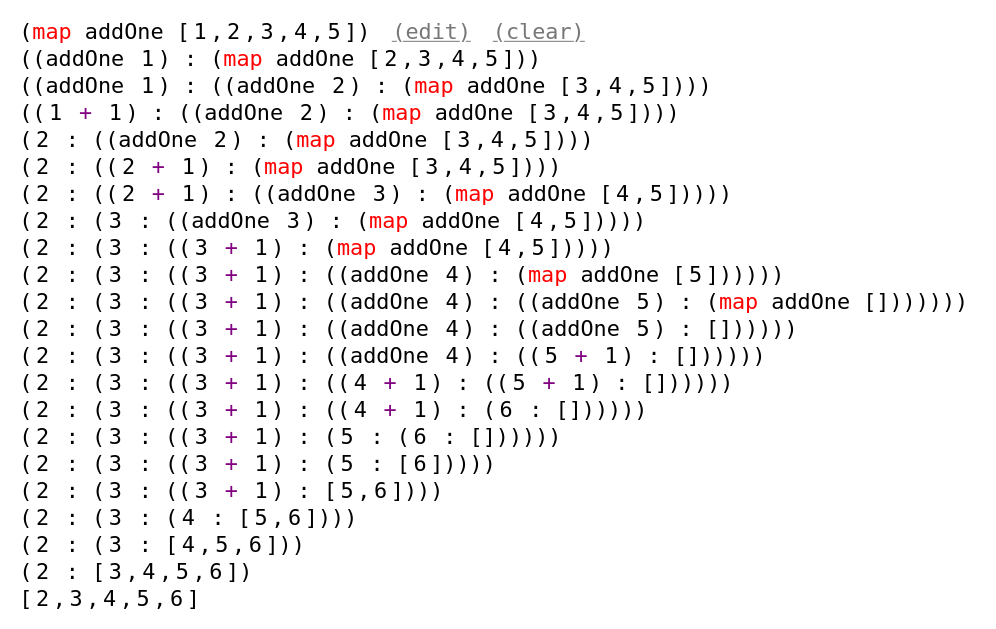
\includegraphics[width=0.75\linewidth]{images/LLessonsMap.png}
    \caption{Evaluation of\ `\sflinline{map addOne [1, 2, 3, 4, 5]}'\ with \llessons}
    \label{bg:llessons_ui}
\end{figure}

\begin{figure}[t]
    \centering
    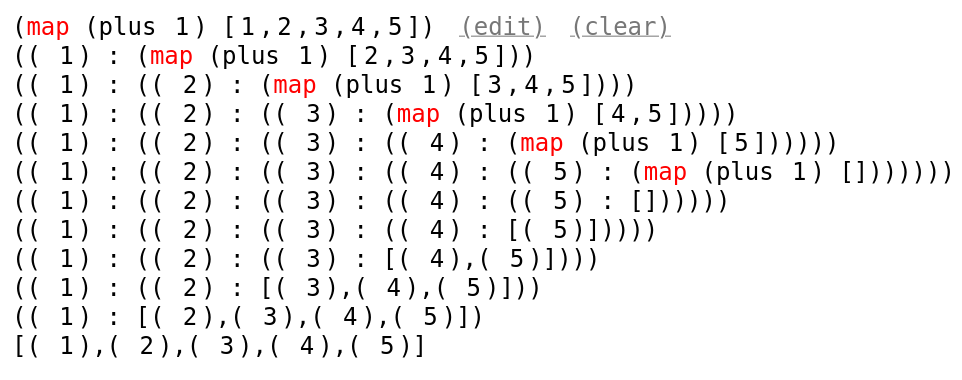
\includegraphics[width=0.75\linewidth]{images/LLessonsGoingWrong.png}
    \caption{Evaluation of `\sflinline{map (plus 1) [1, 2, 3, 4, 5]}' with \llessons. It gets confused by currying and partial application}
    \label{bg:llessons_gets_confused}
\end{figure}

The UX/UI is the definite strong point of \llessons (see \ref{bg:llessons_ui}).  However, there are a few things that I would identify as weaknesses that make it not useful for what SFL explorer is useful for. 

\begin{itemize}
    \item The language is not typechecked. There are type assignments, but upon testing and inspection of the source code \cite{lambdalessonsgithub}, type assignments are ignored. 
    \item The language does not allow for user defined algebraic data types, but it has \sflinline{List} built in. 
    \item As can be seen in \ref{bg:llessons_ui}, it seems to imply that \sflinline{((x : y : []))} reduces to \sflinline{[x, y]} which is misleading. 
    \item The language does not support lambda functions
    \item The language does not support currying (\ref{bg:llessons_gets_confused})
    \item The program states are not saved between refreshes.
\end{itemize} 

In summary, \llessons\ is designed for a different purpose than SFL Explorer. It describes itself as a `document' \cite{lambdalessons} rather than a tool, which is an apt description as it is a document meant to teach one specific thing rather than to be an all around teaching tool for functional languages. It does not provide much of a capability to experiment yourself as the language is not very extensive. However, the ability to reduce an expression by clicking on the bit of the expression you want to reduce is very good, and inspiration should definitely be drawn for future work for SFL Explorer.  

% \subsection{Other Notable Mentions}
% Unfortunately, I do not have the page count to spare to go into detail about some of the other existing systems identified. Here are some of my favorites, along with a brief summary of their achievements. 

% \begin{itemize}
%     \item WinHIPE \cite{WinHIPE}
% \end{itemize}

% \subsection{Conclusion of Research on Existing Systems}


% https://stevekrouse.github.io/hs.js/